\documentclass[a4paper]{beamer}
%
% Josef Hlavac & Tomas Zahradnicky (21.10.2010)
%
%\usepackage{pgfpages}
%\pgfpagesuselayout{4 on 1}[a4paper,border shrink=5mm,landscape]
%\pgfpagesuselayout{resize}[a4paper,border shrink=5mm,landscape]
%\usepackage[czech]{babel}
\usepackage[utf8]{inputenc}
\usepackage{color}
\usetheme{Frankfurt}
\useinnertheme{circles}
\usepackage{subfigure}
\usepackage[czech]{babel}%\useinnertheme{rounded}
%\useinnertheme{rectangles}
%\useinnertheme{balls}
\usefonttheme{professionalfonts}
%
\def\uv#1{\char92\relax #1\char34\relax}
%%%%%%%%%%%%%%%%%%%%%%%%%%%%%%%%%%%%%%%%%%%%%%%%%%%%%%%%%%%%%%%%%%
\newcommand\PersonTitle{Bc.}
\newcommand\FirstName{Jan}
\newcommand\FirstNameAbbreviated{J}
\newcommand\LastName{Jeníček}
\newcommand\Email{jenicja2@fit.cvut.cz}
\newcommand\DissertationTitle{Frontend webové aplikace na učení se programování}
%\newcommand\Department{Department of Theoretical Computer Science}
%\newcommand\Department{Department of Digital Design}
%\newcommand\Department{Department of Software Engineering}
%\newcommand\Department{Department of Computer Systems}
%\newcommand\Faculty{Faculty of Information Technology}
%\newcommand\University{Czech Technical University in Prague}
%\newcommand\FacultyAndUniversityAbbr{FIT CTU}
%%%%%%%%%%%%%%%%%%%%%%%%%%%%%%%%%%%%%%%%%%%%%%%%%%%%%%%%%%%%%%%%%%
%\subtitle{BBB}
%\subject{SUBJECT}
\author[\PersonTitle{} \FirstNameAbbreviated. \LastName]{\PersonTitle{} \FirstName{} \LastName}
\title{\DissertationTitle}
%\titlegraphic{
\includegraphics[width=1.5cm]{pic/LogoCVUT.pdf}}
%\institute[\FacultyAndUniversityAbbr]{\Department\\ \Faculty\\ \University}
% Write - sem dát datum kdy to budu prezentovat při obhajobě 
\date{11.~června~2026}
%
\begin{document}
\begin{frame}
%\begin{center}
%
\includegraphics[width=1.5cm]{pic/LogoCVUT.pdf}
%\end{center}
\titlepage
\end{frame}

% Write - tenhle slide možná vyřadit?
%\section*{Obsah}
%\subsection*{Obsah}
%\begin{frame}
%\frametitle{Obsah}
%\tableofcontents
%\end{frame}

% Done
\section{Úvod}
\subsection*{Motivace}
\begin{frame}
\frametitle{Motivace}
\begin{itemize}
\item Neuspokojivé aplikace na výuku angličtiny
\begin{itemize}
    \item Efektivita učení
    \item Zábavnost učení
    \item Přizpůsobitelnost učení
\end{itemize}
\item Rozdělení projektu
\begin{itemize}
    \item Frontend
    \item Backend
\end{itemize}
\end{itemize}
\end{frame}

% Done
\subsection*{Cíle práce}
\begin{frame}
\frametitle{Cíle práce}
\begin{enumerate}
\item Hlavní cíl: Vytvoření a nasazení frontendu aplikace
\begin{itemize}
\item Analýza
\item Návrh
\item Implementace
\item Testování
\item Nasazení
\item Zhodnocení
\end{itemize}
\end{enumerate}
\end{frame}

% Done
\section{Řešení}
\subsection*{Analýza}
\begin{frame}
\frametitle{Analýza}
\begin{enumerate}
    \item Analýza existujících řešení
    \begin{itemize}
        \item Použitelnost, učení, motivace, silné a slabé stránky
        \item Duolingo, Mondly, Busuu, Babbel
    \end{itemize}
    \item Požadavky aplikace
    \begin{itemize}
        \item Funkční požadavky
        \item Nefunkční požadavky
    \end{itemize}
\end{enumerate}
\end{frame}

% Done
\subsection*{Návrh}
\begin{frame}
\frametitle{Návrh}
\begin{columns}
\begin{column}[c]{4cm}
\begin{enumerate}
\item Případy užití
\item Návrh uživatelského rozhraní
\item Výběr technologií
\end{enumerate}
\end{column}
\begin{column}[c]{6cm}
\begin{figure}[c]
\begin{center}
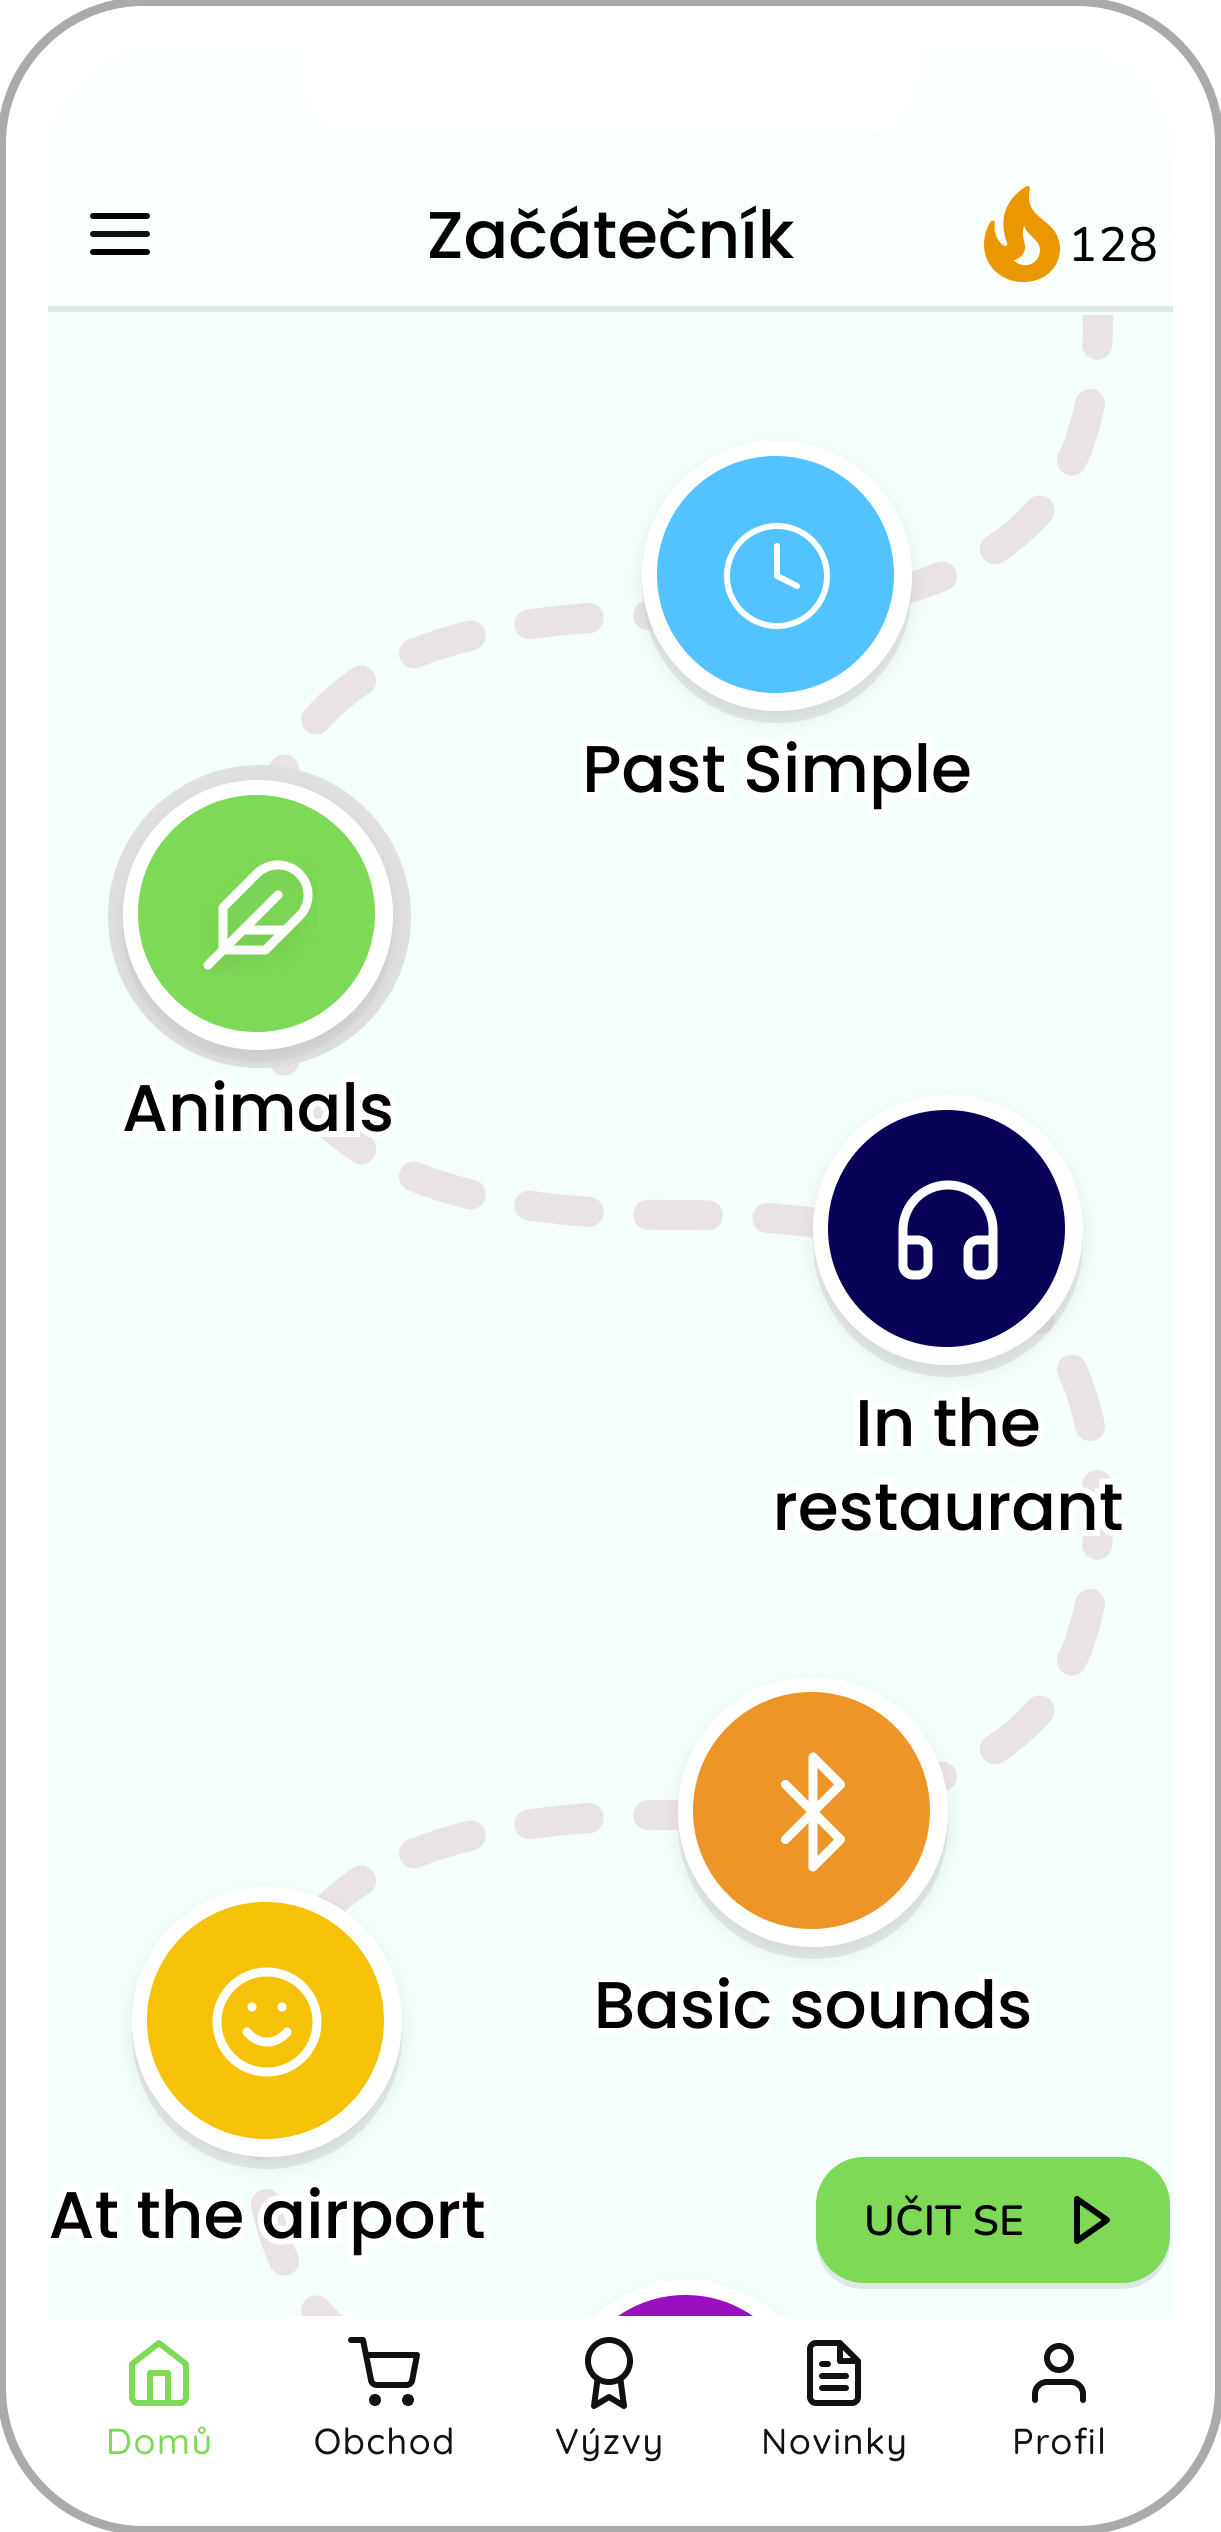
\includegraphics[width=2.9cm]{pic/homepage.png}
\end{center}
\caption{Návrh stránky kurzu}
\end{figure}
\end{column}
\end{columns}
\end{frame}

% Write - tady bych teoreticky ještě mohl přidat jeden slide s dvěma obrázky - lekce a volba témat

% Done
\subsection*{Implementace}
\begin{frame}
\frametitle{Implementace}
\begin{itemize}
    \item Celý návrh byl implementován
    \item React, Next.js a TypeScript % tohle teoreticky můžu vyřadit
    \item Vytvořen Mock API
\end{itemize}
\end{frame}

% Done
\subsection*{Testování}
\begin{frame}
\frametitle{Testování}
\begin{itemize}
    \item Manuální testování
    \begin{enumerate}
        \item Komponenty
        \item Funkce a stránky s mock API
        \item Funkce a stránky s backend API
    \end{enumerate}
    \item Testování použitelnosti
    \begin{itemize}
        \item 5 účastníků
        \item Objeveny příležitosti pro zlepšení UI
    \end{itemize}
\end{itemize}
\end{frame}

% Done
\subsection*{Nasazení}
\begin{frame}
\frametitle{Nasazení}
\begin{itemize}
    \item Testovací prostředí využívající mock REST API
    \item Produkční prostředí využívající backend API
    \item Aplikace je připravena k provozu
\end{itemize}
\end{frame}

% Done
\section{Závěr}
%\subsection*{Budoucí vývoj}
%\begin{frame}
%\frametitle{Budoucí vývoj}
%\begin{itemize}
%    \item Automatizované testování
%    \item Zdokonalení stávajících funkcí
%    \item Vytvoření PWA
%\end{itemize}
%\end{frame}

% Done
\subsection*{Závěr}
\begin{frame}
\frametitle{Závěr}
\begin{itemize}
\item Byl vytvořen a nasazen frontend aplikace
\item Aplikace je připravena k provozu
\item Vývoj aplikace bude pokračovat
\end{itemize}
\end{frame}

% Done
\section*{Diskuze}
\subsection*{Diskuze}
\begin{frame}
\begin{center}
\vspace*{1cm}
{\bf Děkuji za pozornost!}\\
\vspace*{2cm}
{\bf\Large \PersonTitle{} \FirstName{} \LastName{}}\\
{\tt \Email}
\vspace*{1cm}
\end{center}
\vfill
% {\tiny {\bf Acknowledgement:} This research has been partially supported by the Ministry of Education, Youth, and Sport of the Czech Republic under research program MSM 6840770014. \fcolorbox{black}{green}{IF \the\day.\the\month.\the\year{} $\geq$ 31.12.2011 UPDATE MSM 6840770014}.}
\end{frame}
%
\appendix
\section{Otázka 1}
\subsection{Otázka 1}
\begin{frame}
\begin{block}{Otázka 1}
    Nezkoušel jste z Figmy pomocí AI rovnou vygenerovat celou funkční aplikaci? Jak to případně dopadlo?
\end{block}
\end{frame}

\end{document}
